\documentclass[conference]{IEEEtran}
\usepackage[T1]{fontenc}
\usepackage[utf8]{inputenc}
\usepackage{amsmath,amssymb,booktabs,graphicx,array,url}
\usepackage[hidelinks]{hyperref}
\graphicspath{{figures/}}
\newcommand{\AP}{\operatorname{AP}}
\newcommand{\reportauthors}{\begin{tabular}{lc}Mohammed Ali Hossain & 21301453\\[0.3em]Jarin Akter Mou & 20301070\\[0.3em]Asiful Kanzan Auishik & 19101628\end{tabular}}
\newcommand{\reportinstitution}{BRAC University}
\begin{document}
\onecolumn
\begin{titlepage}
\centering
\vspace*{1.2cm}
{\Large Neural Networks Project Report\par}
\vspace{1.2cm}
{\LARGE\bfseries GNN-Based BERT for Understanding Context from Music\par}
\vspace{0.7cm}
{\large Supervised Context Tagging and Contrastive MusicCaps Alignment\par}
\vspace{1.3cm}
{\large\reportauthors\par}
\vspace{0.5cm}
{\large\reportinstitution\par}
\vspace{0.8cm}
{CSE715\par}
{12 September 2026\par}
\vspace{1.1cm}
\begin{minipage}{0.88\textwidth}
\section*{Abstract}
This project evaluates whether graph representations of audio improve music-context prediction beyond a strong caption-based BERT baseline. A single canonical MusicCaps dataset of 5,140 usable clips supports four connected tasks: text classification, audio-only CNN and graph classification, supervised GNN--BERT fusion, and contrastive audio--caption alignment. Experimental discipline is central: splits precede TRAIN-only label construction, preprocessing artifacts are hash-locked, validation selects models, and final TEST protocols freeze seeds and evaluation rules. Fine-tuned BERT achieves validation Macro Average Precision (AP) of 0.841, compared with 0.229 for the strongest audio-only CNN. On three-seed TEST evaluation, Early Fusion reaches 0.8319 Macro AP versus 0.8313 for BERT; the difference of +0.00058 changes sign across seeds and its exploratory bootstrap interval includes zero. Thus, fusion does not establish a reliable overall advantage. Contrastive retrieval reaches mean recall of $0.0796\pm0.0065$, approximately $7.7\times$ random retrieval over 514 candidates, although exact-pair recall at one remains about 2\%. Five listeners rating ten fixed queries produce a pooled mean of 3.02/5 with substantial variability. Prototype-based tag readout is weaker than supervised classification and inherits encoders previously trained on the same labels. Caption--label overlap, unverified recording-level duplicate isolation, and the small listening study constrain interpretation. The principal contribution is a reproducible comparison that identifies both useful cross-modal alignment and the limits of the implemented fusion approach.
\end{minipage}
\vfill
\end{titlepage}
\twocolumn
\pagestyle{plain}
\setcounter{tocdepth}{1}
\tableofcontents
\section{Introduction and Motivation}\label{sec:intro}
Musical context includes instrumentation, tempo, mood, and production quality. We evaluate graph--text models on one frozen MusicCaps dataset and shared label vocabulary.

The resulting experiment addresses three questions. First, how predictive are caption, spectrogram, and segment-graph representations for the same 20 labels? Second, does supervised graph--text fusion improve upon BERT alone? Third, can contrastive training align audio and captions sufficiently to support retrieval and label-prototype readout? These questions distinguish classification from cross-modal correspondence: a strong caption classifier need not imply a strong audio retriever.

All four assignment stages are implemented. The independent audit documents the controlled experimental chain supporting the reported comparisons.

\section{Related Work and Background}\label{sec:background}
BERT learns contextual text representations through bidirectional language-model pretraining and supports task adaptation with a classification head~\cite{bert}. Here it encodes human-authored music captions, not transcribed lyrics. GraphSAGE aggregates neighborhood features to construct inductive graph representations~\cite{sage}; GAT instead learns attention weights within graph neighborhoods~\cite{gat}. Both provide appropriate mechanisms for testing whether local temporal links and segment similarity help summarize music clips. Learned attention weights, however, are not automatically explanations of musical structure.

InfoNCE trains representations by discriminating matched examples from alternatives~\cite{cpc}. CLIP demonstrates paired encoders trained with a symmetric cross-modal contrastive objective~\cite{clip}. This project applies that objective pattern to audio graphs and captions; it does not use CLIP weights or claim comparable scale. MusicCaps supplies musician-written captions and aspect lists for short audio clips~\cite{musiccaps,musiclm}. Its paired annotations enable all four tasks, but their semantic relationship also creates a potential shortcut in caption-to-tag prediction.

\section{Problem Formulation}\label{sec:problem}
Following the assignment, a track is represented as
\begin{equation}
T=(X_{\mathrm{audio}},X_{\mathrm{text}},G,y),\quad y\in\{0,1\}^{20},
\label{eq:tuple}
\end{equation}
where $G=(V,E)$ connects audio segments. The context target in~\eqref{eq:tuple} is multi-label tagging; no emotion-regression objective is evaluated. The text encoder produces $H_{\mathrm{text}}\in\mathbb{R}^{112\times768}$ and its CLS vector $t$. A generic graph layer updates node $i$ through
\begin{equation}
h_i^{(\ell+1)}=\phi\!\left(W^{(\ell)}\operatorname{AGG}\left(h_i^{(\ell)},\{h_j^{(\ell)}:j\in\mathcal N(i)\}\right)\right).
\label{eq:message}
\end{equation}
GraphSAGE instantiates~\eqref{eq:message} with concatenation of the node state and mean neighbor state; GAT uses attention-weighted neighbor aggregation. Mean pooling yields
\begin{equation}
g=|V|^{-1}\sum_{i\in V}h_i^{(L)},\quad z=\operatorname{Fusion}(g,t),\quad \hat y=\sigma(Wz+b).
\label{eq:readout}
\end{equation}
The task-specific readouts in~\eqref{eq:readout} optimize binary cross-entropy over the 20 labels, with positive weighting in the audited supervised pipeline. In generic weighted form,
\begin{equation}
\mathcal L_{\mathrm{tag}}=-\frac1{20}\sum_{k=1}^{20}\left[w_k y_k\log\hat y_k+(1-y_k)\log(1-\hat y_k)\right].
\label{eq:bce}
\end{equation}
The report does not infer unprovided numerical class weights.

For contrastive learning, projections of $g_i$ and $t_i$ are normalized into $a_i,c_i\in\mathbb R^{256}$. With $s_{ij}=a_i^\top c_j/\tau$, the symmetric objective is
\begin{equation}
\mathcal L_{\mathrm{NCE}}=-\frac1{2B}\sum_{i=1}^{B}\left[\log\frac{e^{s_{ii}}}{\sum_j e^{s_{ij}}}+\log\frac{e^{s_{ii}}}{\sum_j e^{s_{ji}}}\right].
\label{eq:nce}
\end{equation}
Equation~\eqref{eq:nce} uses $B=32$ and $\tau=0.07$. The diagonal encodes true pairs, while other batch items serve as negatives.

\section{Dataset and Preprocessing}\label{sec:data}
\subsection{Acquisition and canonical split}
The initial metadata contained 5,521 unique track and source IDs, with no missing captions or aspect lists. A deterministic 200-track audit at seed 42 yielded 188 usable clips. Some approximately 20-second downloads were investigated for temporal alignment; the intended interval lay in the final approximately ten-second region for affected artifacts. Full acquisition initially recovered 4,847 clips and controlled recovery increased this to 5,140. Table~\ref{tab:data} records the final dataset boundary.
\begin{table}[t]
\caption{Audited dataset and feature specification.}\label{tab:data}
\centering\small
\begin{tabular}{@{}ll@{}}\toprule
Property & Frozen value\\\midrule
Metadata / usable / excluded & 5,521 / 5,140 / 381\\
Acquisition yield & 93.10\%\\
TRAIN / VAL / TEST & 4,112 / 514 / 514\\
Split seed / vocabulary & 42 / Top-20\\
Waveform & 22,050 Hz, mono, 10.0 s\\
Samples per clip & 220,500\\
Log-mel / chroma & $128\times431$ / $12\times431$\\
FFT / hop length & 2,048 / 512\\
Tokens / TRAIN truncation & 112 / 1.43\%\\
Graph windows / stride & 2 s / 1 s\\
Nodes / raw node dimension & 9 / 140\\\bottomrule
\end{tabular}
\end{table}

The split was frozen before vocabulary construction. Track/source identity overlap was checked, but artist and recording near-duplicate isolation was not independently established. All tasks retain the same canonical MusicCaps examples. This supports cross-task comparability while deviating from the assignment's specific Task-2/3 references to GTZAN, FMA, or MagnaTagATune. Those datasets were not used, and results on them are not claimed.

\subsection{Text and labels}
Multiword aspects were preserved, normalized, conservatively synonym-merged, and frequency-filtered using TRAIN only before freezing the Top-20 vocabulary. The full label order appears in Appendix~\ref{sec:appendix}. The target is a caption-to-aspect proxy task for text models. The degree of direct phrase or synonym overlap between captions and labels was not measured.

Tokenization uses \texttt{bert-base-uncased}. The TRAIN 95th-percentile length was 97 tokens; the chosen maximum of 112 gave 1.43\% TRAIN truncation. This empirical choice replaces the assignment's suggested 128--256 range. The frozen token cache contains input IDs, attention masks, and token-type IDs of shape $(5140,112)$. Applying the fixed tokenizer to TEST during preprocessing is distinct from using TEST labels or metrics for model selection.

\subsection{Audio features and graph construction}
Accepted waveforms were standardized as in Table~\ref{tab:data}. Log-mel features were normalized within each track; chroma supported cosine-based topology. Nine overlapping two-second windows provide node features comprising 128 mean mel values and 12 mean chroma values. A model-side linear layer maps 140 dimensions to 64.

G1 connects consecutive nodes bidirectionally, giving 16 directed edges. Initial G2 added all chroma-similar pairs above 0.85 and could degenerate into a complete 72-edge directed graph. A 100-TRAIN-track structural study showed that increasing the threshold alone did not adequately prevent density. Before formal graph training, G2 was amended to retain temporal edges and add nonlocal similarity pairs above 0.85 in strongest-first order, with at most two additional similarity neighbors per node. Edges are bidirectional; the final cache averages roughly 30 directed edges and caps at 34. The cap preserves sparse nonlocal connectivity without replacing temporal structure. It was a pre-result structural correction, not a TEST-driven choice.

Figure~\ref{fig:graph} shows the supplied hard-case graph: nine nodes, eight temporal and five additional undirected edges. This is a topology illustration, not a visualization of learned attention or proof of chord-level reasoning.
\begin{figure}[t]\centering
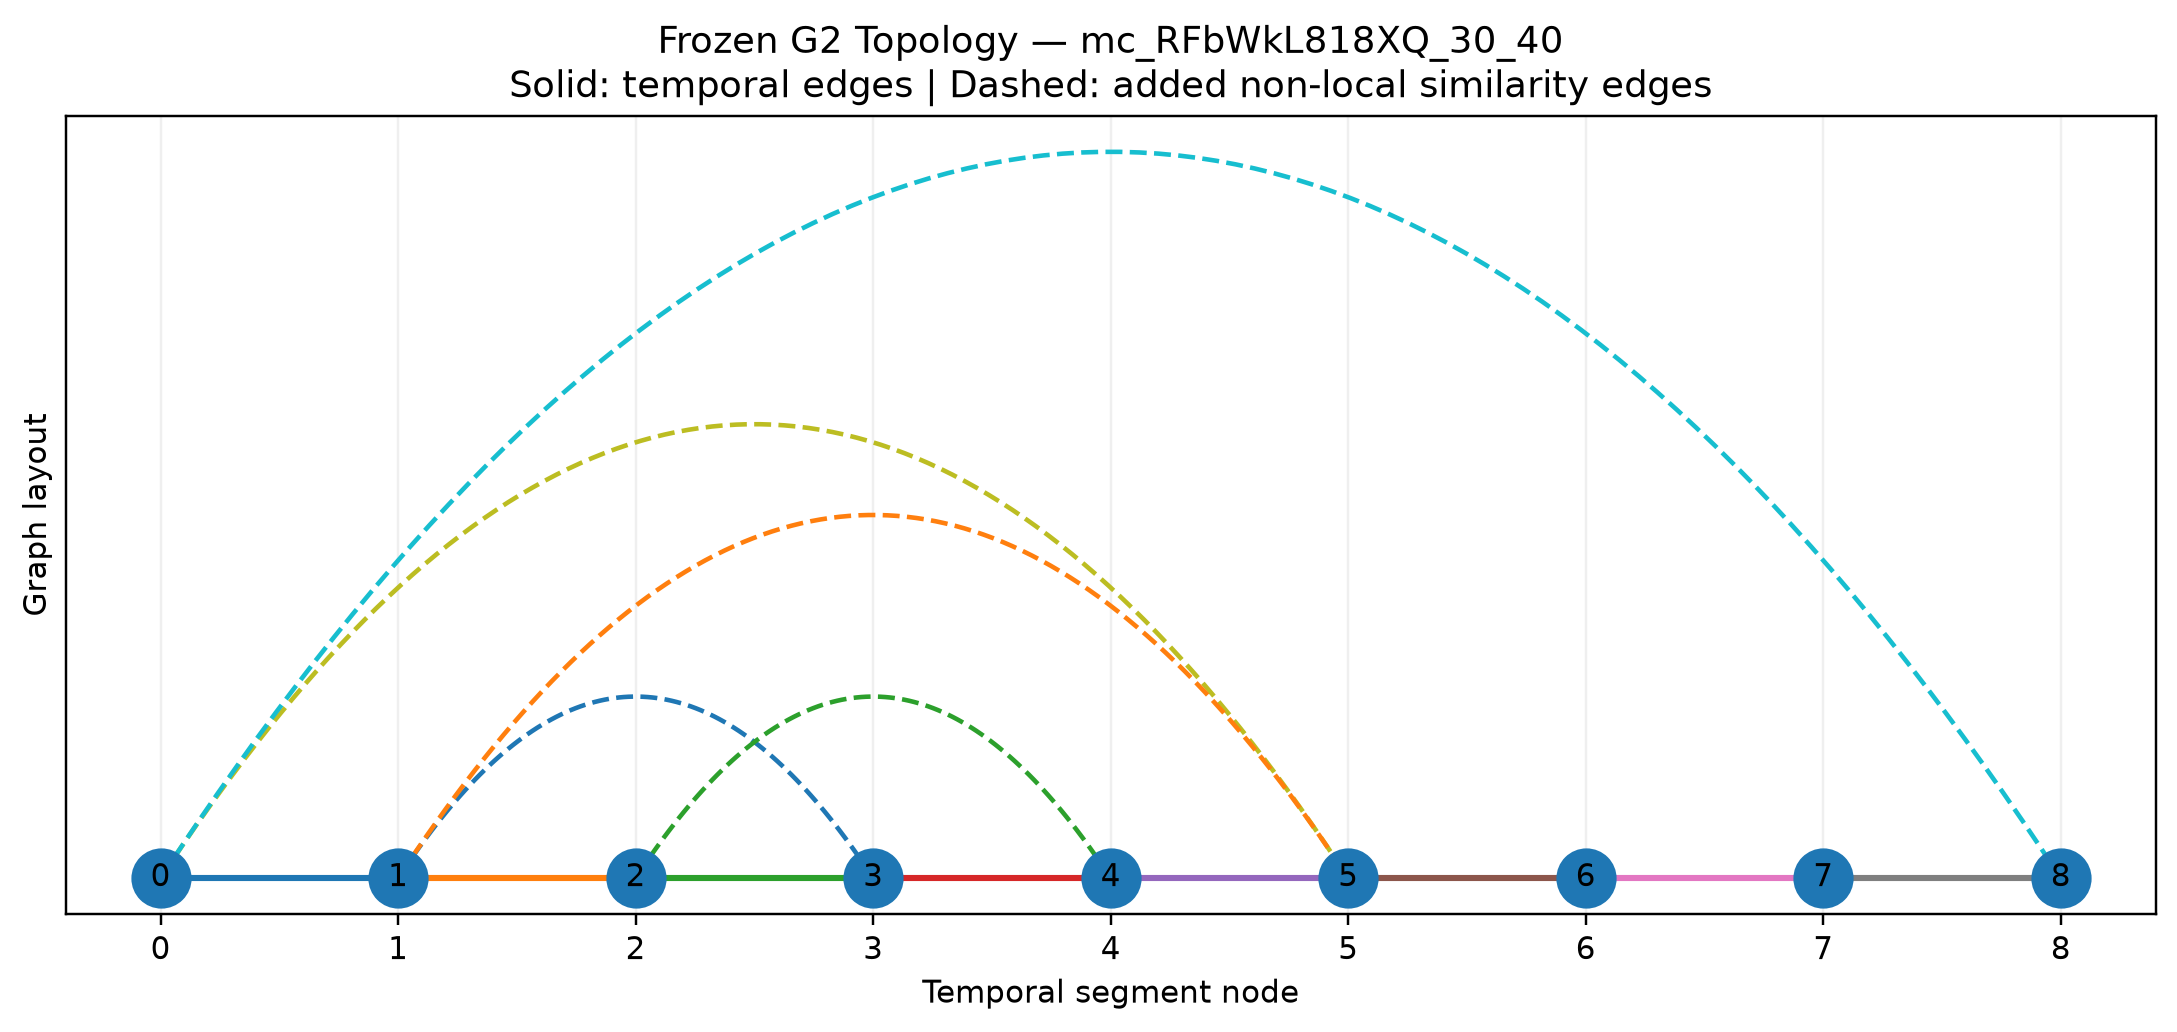
\includegraphics[width=\linewidth]{figure_G2_hard_case_graph.png}
\caption{Supplied G2 example for track \protect\texttt{mc\_RFbWkL818XQ\_30\_40}. Temporal and sparse nonlocal links connect mean-pooled audio segments.}\label{fig:graph}
\end{figure}

\section{Methodology}\label{sec:methods}
\subsection{Task 1: BERT baseline}
T1-A freezes BERT and trains a linear classification head. T1-B fine-tunes the full encoder, using the final hidden-state CLS vector, dropout, and a $768\to20$ classifier. TRAIN supplies optimization examples and VAL selects the checkpoint by Macro AP; TEST is excluded from development. T1-B is selected at epoch 8. The distinction between frozen and fully fine-tuned BERT tests adaptation to the project vocabulary rather than comparing unrelated text models.

\subsection{Task 2: Audio-only models}
A1 is a CNN over mel-spectrograms. A2 and A3 use GraphSAGE over G1 and G2 respectively; A4 uses GAT over G2. The selected GAT has a $140\to64$ node projection, two attention layers with four concatenated 32-dimensional heads (128 outputs), and a third four-head layer producing 128 outputs with \texttt{concat=False}. Global mean pooling feeds a $128\to20$ classifier. Attention dropout is 0.2, self-loops are used, and no explicit residual path is present.

The overall audio winner and selected graph encoder are separate decisions: CNN wins audio classification, while A4 is selected among graph candidates for fusion. GAT/G1 was not formally evaluated. Consequently, a G2 benefit for GraphSAGE does not demonstrate the same benefit for GAT. The CNN reaches its best development result at the epoch-15 ceiling; the frozen budget is retained.

\subsection{Task 3: GNN--BERT fusion}
Early Fusion M3 projects BERT CLS from 768 to 256 dimensions and the pooled GAT vector from 128 to 256. Concatenation produces 512 dimensions, followed by a $512\to256$ layer, dropout 0.2, and a $256\to20$ output. This instantiates the fusion readout of~\eqref{eq:readout} using complementary global summaries.

M4 projects the pooled graph vector into a graph-level query over the BERT sequence. In compact notation,
\begin{equation}
Q=gW_Q,\quad K=H_{\mathrm{text}}W_K,\quad A=\operatorname{softmax}(QK^\top/\sqrt d).
\label{eq:attention}
\end{equation}
The attended text representation in~\eqref{eq:attention} supports the final fused readout. Because $g$ is already pooled, this is graph-level-to-token cross-attention, not node-to-token alignment.

Phase A uses frozen TRAIN+VAL representations: BERT sequences have shape $(4626,112,768)$ and GAT embeddings $(4626,128)$, aligned by track ID with no TEST rows. Neither candidate surpasses the BERT reference, activating the predefined Phase-B refinement gate. Phase B improves both fusion candidates, and M3 is selected on VAL. Exact Phase-B layer scope and optimizer settings cannot be fully reconstructed from the supplied final audit and result export; this report does not invent them. Final variability must therefore be interpreted with the audit's warning about potentially shared upstream checkpoints.

\subsection{Task 4: Contrastive alignment and readout}
The dual encoder projects BERT CLS and pooled GAT features into a shared normalized 256-dimensional space and optimizes~\eqref{eq:nce}. T4-A trains projection heads with encoders frozen. T4-B initializes from T4-A projections and the original T1-B/A4 encoders, then trains BERT layers 10--11, GAT3, and both projections. BERT embeddings/layers 0--9, the GAT input projection, GAT1/GAT2, and the old classification head remain frozen. Frozen parameters need not imply deterministic activations when training-mode dropout remains active.

Validation mean recall selects T4-B before TEST. Retrieval then uses normalized cosine similarity without post-hoc reranking, best-seed selection, or ensembling. Canonical label phrases are embedded as prototypes, and caption or audio embeddings are scored against them for tag readout. No additional Task-4 tag-supervised optimization or TEST prompt engineering is performed. Nevertheless, upstream T1-B/A4 training used the same 20 labels. The experiment is therefore \emph{prototype-based tag readout after supervised encoder initialization}, not strict label-naive zero-shot learning.

For human evaluation, ten query indices and seed 42 were fixed before inspecting TEST retrieval. The listening study uses the top-one audio retrieval for each fixed caption query. The supplied HTML asks listeners to read each caption, hear the complete clip, and independently assign one rating: 1 no match, 2 weak match, 3 moderate match, 4 good match, or 5 excellent match. It requires a listener ID and all ten ratings before CSV export, but does not technically enforce complete playback. Five listeners provide a complete 50-rating design.

\section{Experimental Setup}\label{sec:setup}
\subsection{Selection, baselines, and metrics}
The final seed set is 42, 1337, and 2026. BERT, CNN, and M3 have three-seed supervised TEST results; GraphSAGE, GAT, and cross-attention are single-seed reporting comparisons. The majority baseline learns each label's majority class from TRAIN and uses TRAIN prevalence as the constant threshold-free score. This separates a trivial prior baseline from the learned models.

Macro Average Precision is the mean of per-label \texttt{average\_precision\_score}, not a claim of trapezoidal precision--recall integration. Macro-F1 averages labelwise F1; Micro-F1 pools decisions globally. Frozen global thresholds are 0.70 for BERT/M3/M4, 0.50 for CNN/GraphSAGE, and 0.45 for GAT. BERT and M3 reach the upper boundary of the predefined 0.30--0.70 grid; F1 results are valid for that protocol, but an unrestricted optimum could lie higher. No TEST threshold extension is made.

For retrieval over $N=514$, the positive rank is one plus the number of candidates with strictly greater similarity. Exact ties do not outrank the positive. Recall at $K$ counts true pairs within the first $K$ positions; $mR$ averages R@1, R@5, and R@10 in both directions. Random ranking gives $mR=(1+5+10)/(3\cdot514)\approx0.0104$. A single query changes directional recall by $1/514\approx0.00195$.

\subsection{Reproducibility and numerical conventions}
Script 29 freezes preprocessing through SHA256 identities. Script 60 first opens target-dependent supervised TEST evaluation after model and threshold selection. Task 4 locks design, selection, multiseed validation, and pre-TEST protocol before Script 72 retrieval evaluation. Subsequent analyses reuse saved outputs. Aborted stale-cache or numerical revalidation attempts are retained as provenance; implementation corrections in Scripts 57, 68, and 70 preceded the relevant TEST access and did not justify changing the frozen scientific choices.

Supervised seed uncertainty uses sample SD ($\mathrm{ddof}=1$); Task-4 seed uncertainty uses population SD ($\mathrm{ddof}=0$). Human pooled and item SDs use sample SD. These quantities describe different sources of variability and are not confidence intervals. Fusion and contrastive seeds may condition on shared supervised initialization; they do not establish variability of independently rebuilt end-to-end pipelines. Final BERT evaluation uses FP16 autocast, whereas the other supervised models use FP32. Exact GPU model, elapsed training time, complete package versions, and Git commit are unavailable in the provided evidence.

\section{Results}\label{sec:results}
\subsection{Tasks 1 and 2: Validation selection}
Table~\ref{tab:selection} gives the audited selection results. Fine-tuning BERT improves VAL Macro AP from 0.559 to 0.841. CNN reaches 0.229, exceeding all evaluated graph candidates; A4 remains the graph choice for downstream tasks. Figure~\ref{fig:training} presents supplied validation curves for the selected text, audio, and fusion pipelines. Legacy plot labels reading ``AUC-PR'' denote Macro AP throughout these supplied figures.
\begin{table}[t]\centering\small
\caption{Tasks 1--2 validation Macro AP.}\label{tab:selection}
\begin{tabular}{@{}lll r@{}}\toprule
Task & Variant & Model/input & Macro AP\\\midrule
1 & T1-A & Frozen BERT + linear head & 0.559\\
1 & T1-B & Full BERT fine-tuning & 0.841\\
2 & A1 & CNN / mel & 0.229\\
2 & A2 & GraphSAGE / G1 & 0.178\\
2 & A3 & GraphSAGE / G2 & 0.184\\
2 & A4 & GAT / G2 & 0.188\\\bottomrule
\end{tabular}
\end{table}
\begin{figure*}[t]\centering
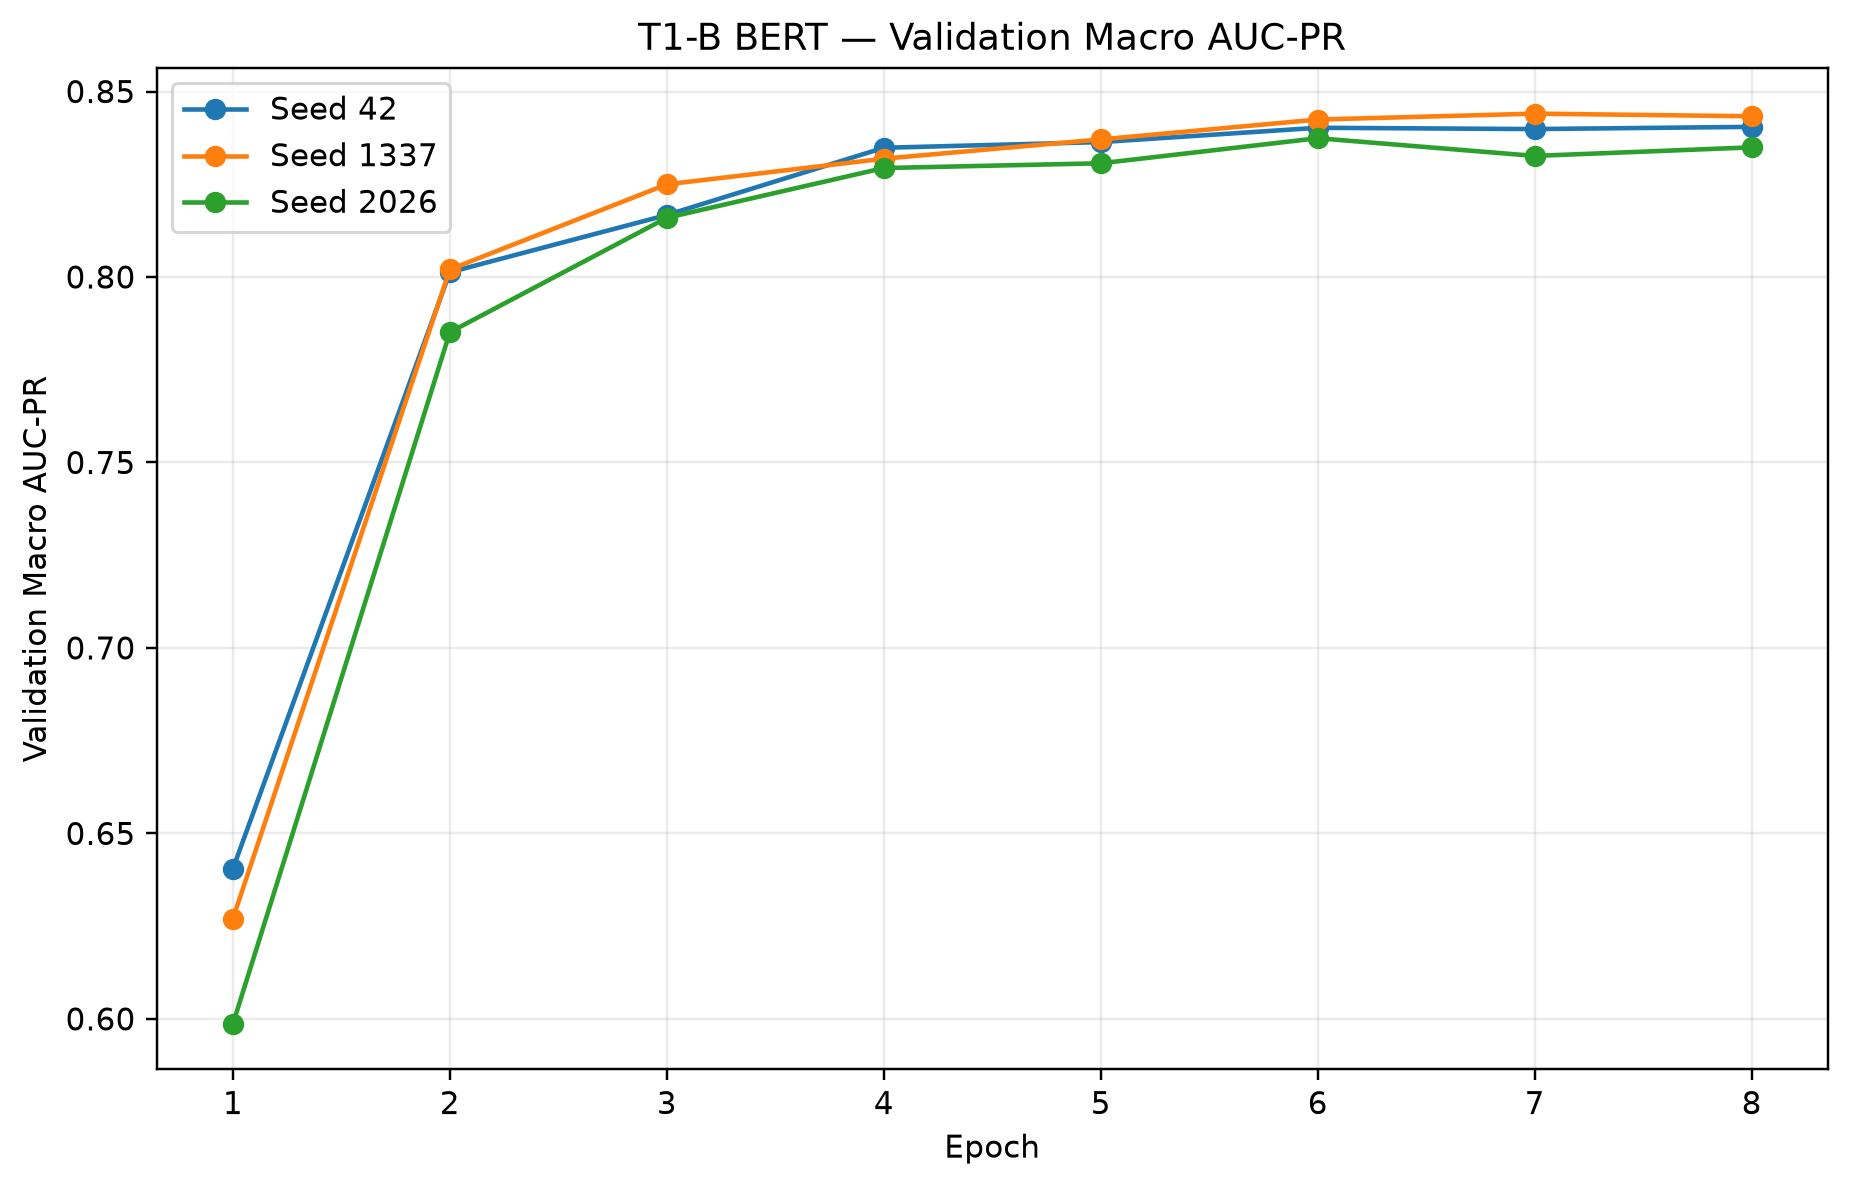
\includegraphics[width=.325\textwidth]{figure_training_T1B.png}\hfill
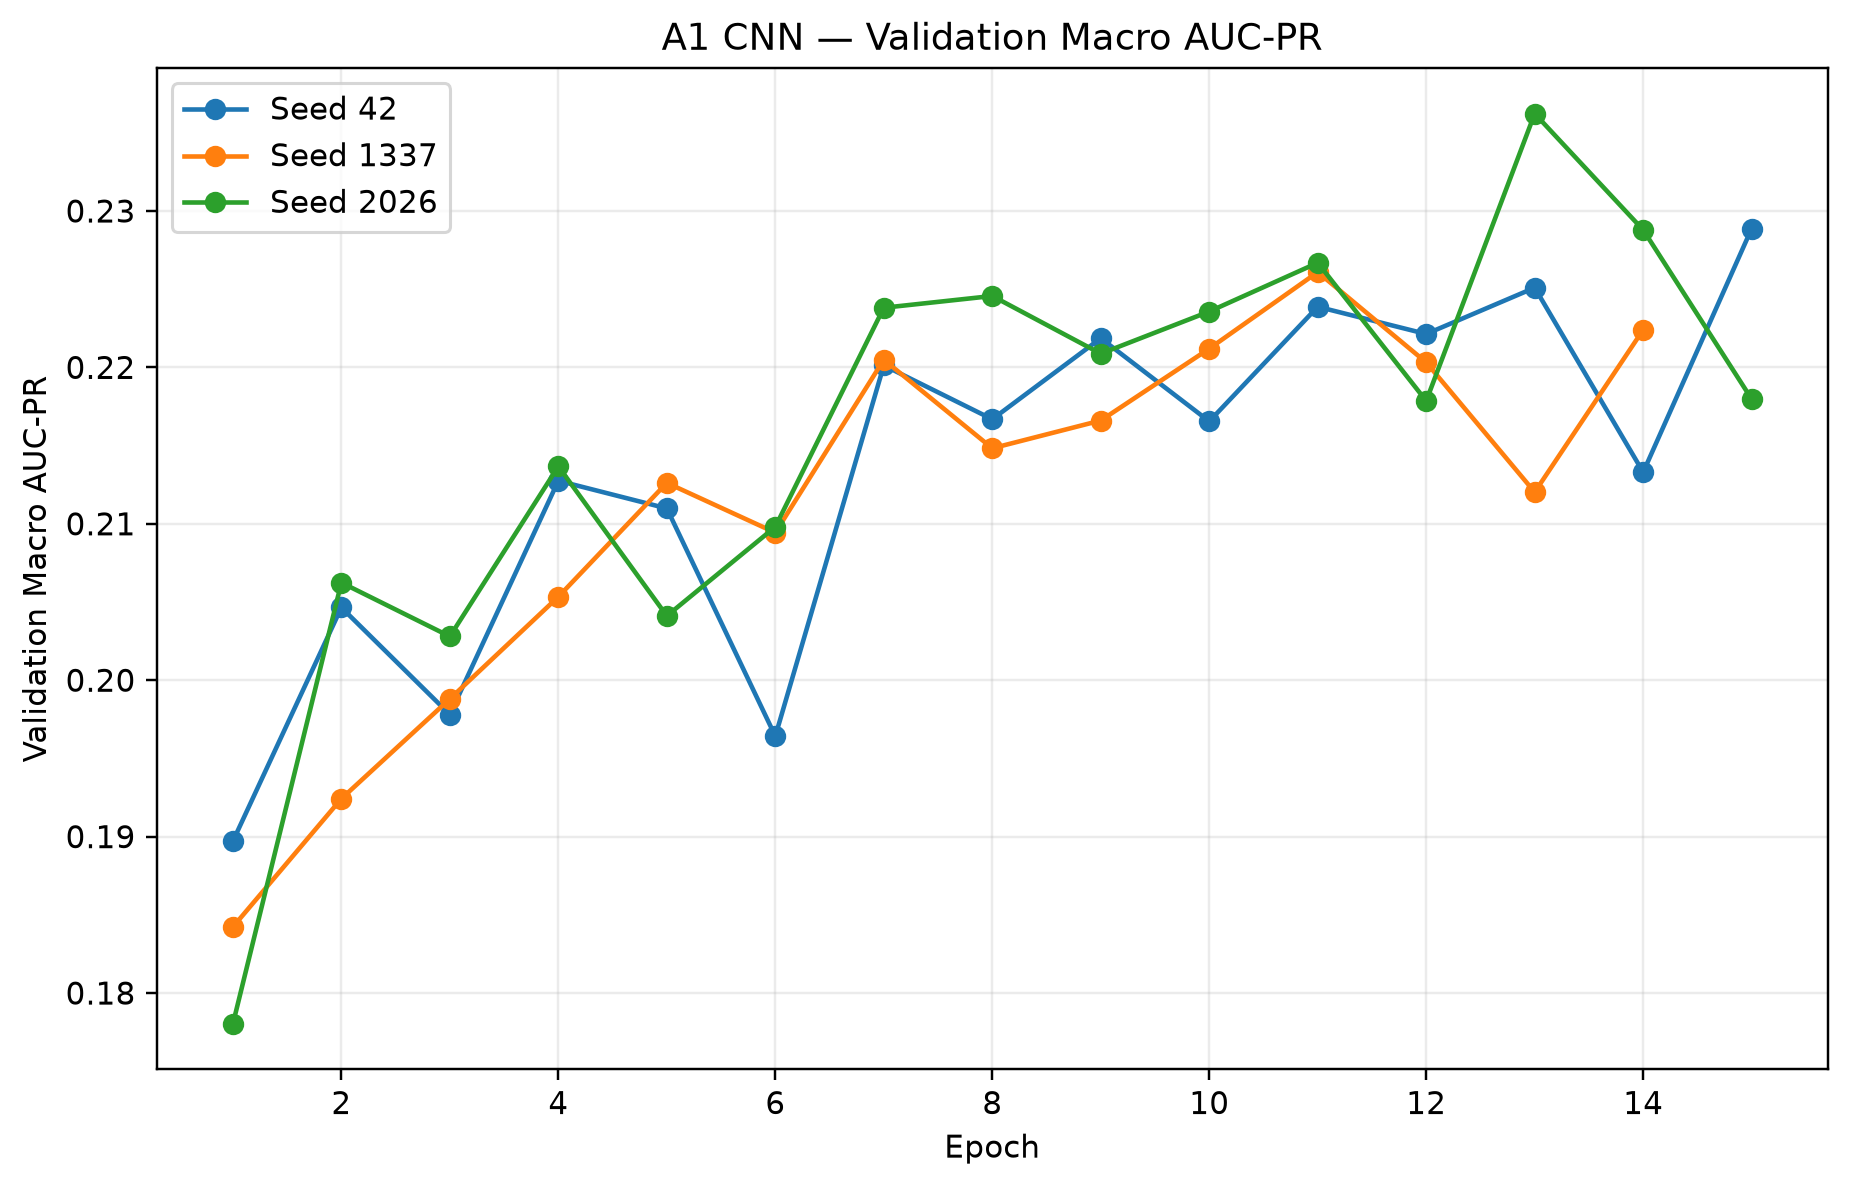
\includegraphics[width=.325\textwidth]{figure_training_A1_CNN.png}\hfill
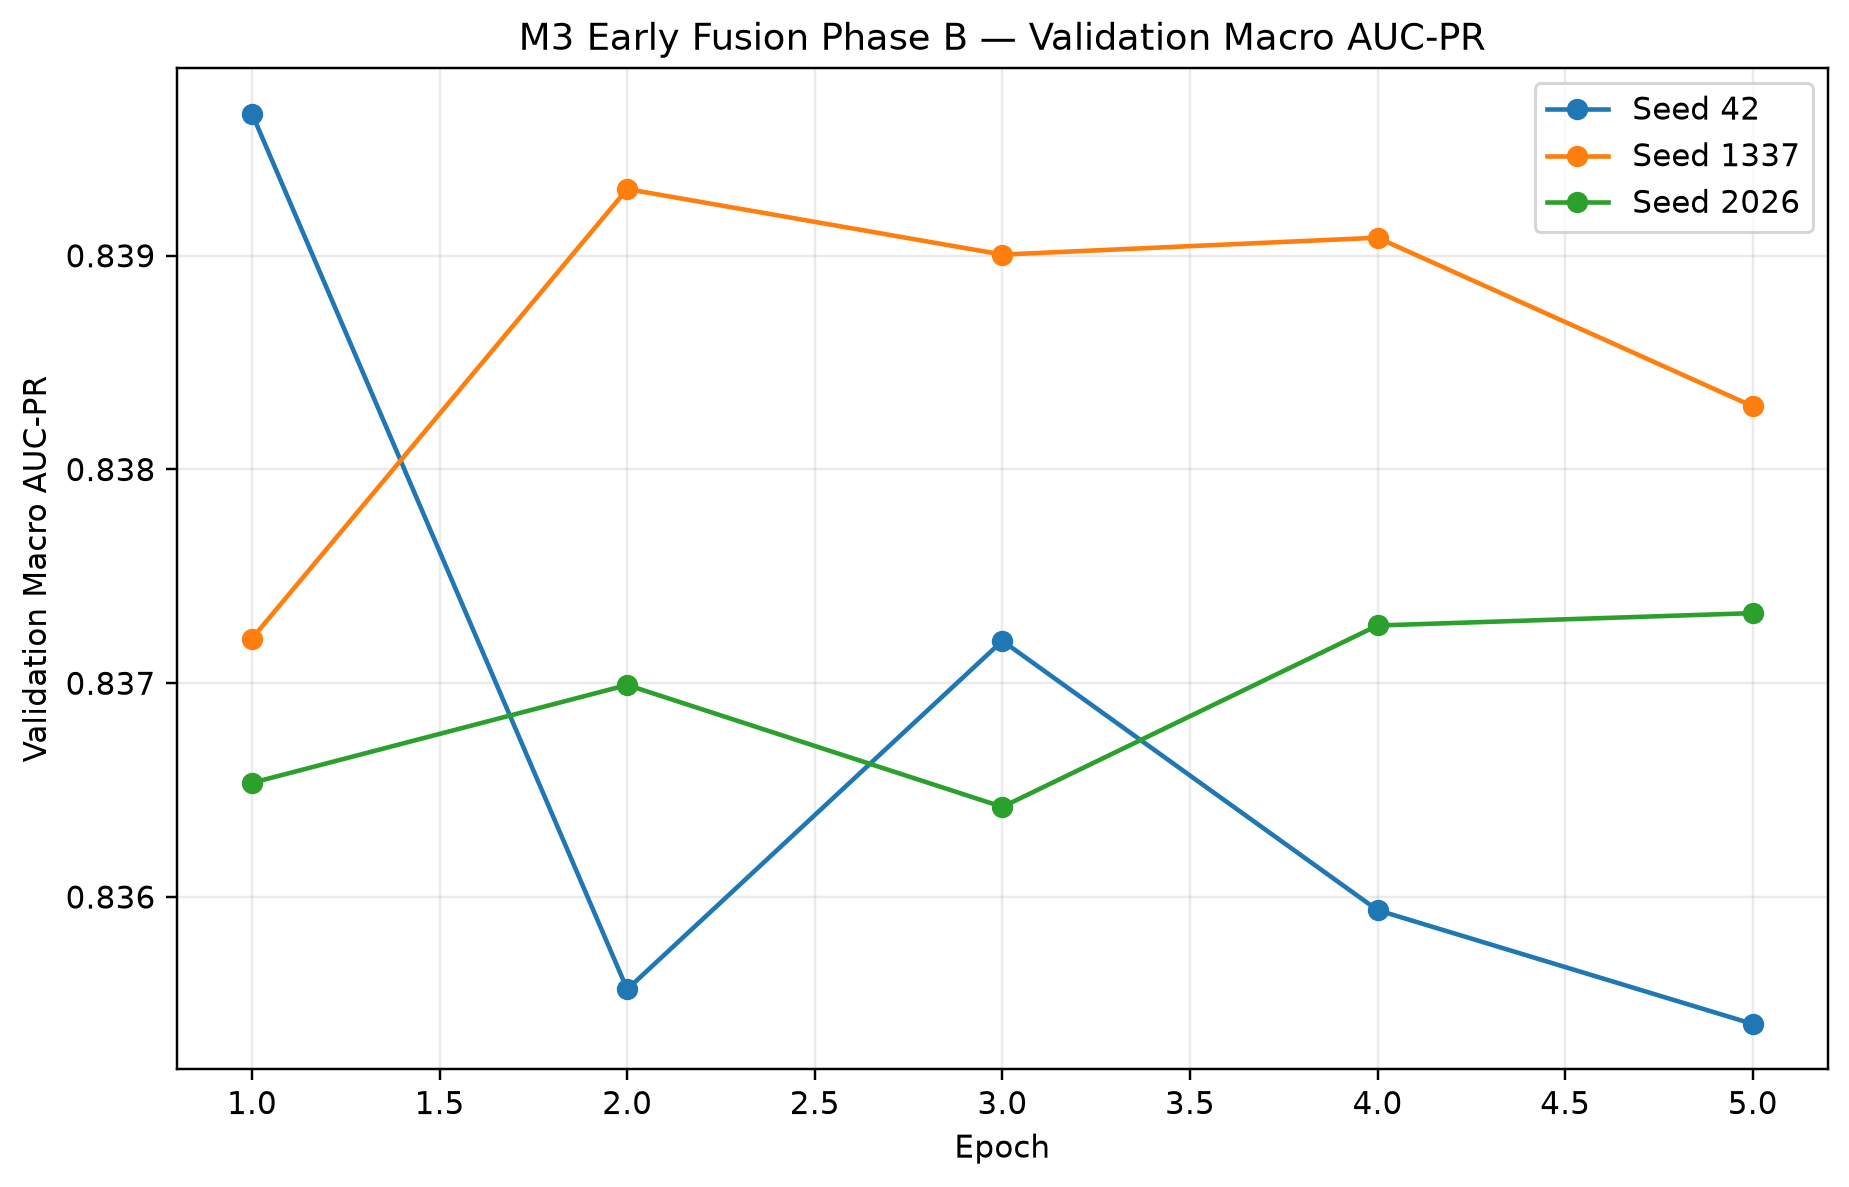
\includegraphics[width=.325\textwidth]{figure_training_M3_phaseB.png}
\caption{Supplied validation Macro AP curves for T1-B (left), A1 CNN (center), and M3 Phase B (right). Plots retain their original metric wording; the implementation measures Average Precision. These are validation trajectories, not repeated TEST selection.}\label{fig:training}
\end{figure*}

\subsection{Task 3: Fusion and final supervised comparison}
Table~\ref{tab:fusionval} distinguishes fusion selection from comparison with the BERT reference. M3 wins over M4 in both phases, but even its Phase-B score remains slightly below the seed-42 BERT validation reference. Winning the fusion comparison does not mean winning the text-versus-fusion comparison.
\begin{table}[t]\centering\small
\caption{Task-3 validation Macro AP from the audit.}\label{tab:fusionval}
\begin{tabular}{@{}lrr@{}}\toprule
Model & Phase A & Phase B\\\midrule
M3 Early Fusion & 0.83072917 & 0.83966470\\
M4 Cross-Attention & 0.82289870 & 0.83215473\\
BERT reference & 0.84057500 & 0.84057500\\\bottomrule
\end{tabular}
\end{table}

The final supervised results in Table~\ref{tab:test} and Figure~\ref{fig:test} show essentially comparable BERT and M3 performance. Their three-seed mean Macro AP values are 0.8313 and 0.8319; the unrounded difference is +0.00058331 (reported as +0.00058). Fusion-minus-BERT differences are $-0.00229684$, $+0.00114464$, and $+0.00290214$ for seeds 42, 1337, and 2026. The exploratory paired-bootstrap 95\% interval is $[-0.00930631,+0.01039828]$. Its inclusion of zero and the sign changes do not support reliable superiority. This is not a formal equivalence test, either.

\begin{table*}[t]\centering\small
\caption{Frozen supervised TEST results. Three-run entries show mean $\pm$ sample SD; one-run entries have no estimated seed SD. Graph models and cross-attention use seed 42. Values from the final evaluation JSON are shown to eight decimal places.}\label{tab:test}
\begin{tabular}{@{}llcrrr@{}}\toprule
Model & Input & Runs & Macro AP & Macro-F1 & Micro-F1\\\midrule
Majority class & TRAIN prior & 1 & 0.10330739 & 0.00000000 & 0.00000000\\
CNN & Audio & 3 & $0.22324414\pm0.00600236$ & $0.27840377\pm0.00487799$ & $0.29176079\pm0.00791052$\\
BERT & Text & 3 & $0.83133318\pm0.00435277$ & $0.78089422\pm0.00965850$ & $0.78079060\pm0.01079046$\\
GraphSAGE & Audio graph & 1 & 0.19439309 & 0.24164746 & 0.26822645\\
GAT & Audio graph & 1 & 0.18767503 & 0.24983767 & 0.27221833\\
Early Fusion & Audio + text & 3 & $0.83191649\pm0.00204706$ & $0.78198704\pm0.00453706$ & $0.78421469\pm0.00410121$\\
Cross-Attention & Audio + text & 1 & 0.82697030 & 0.78351310 & 0.78412560\\\bottomrule
\end{tabular}
\end{table*}
\begin{figure}[t]\centering
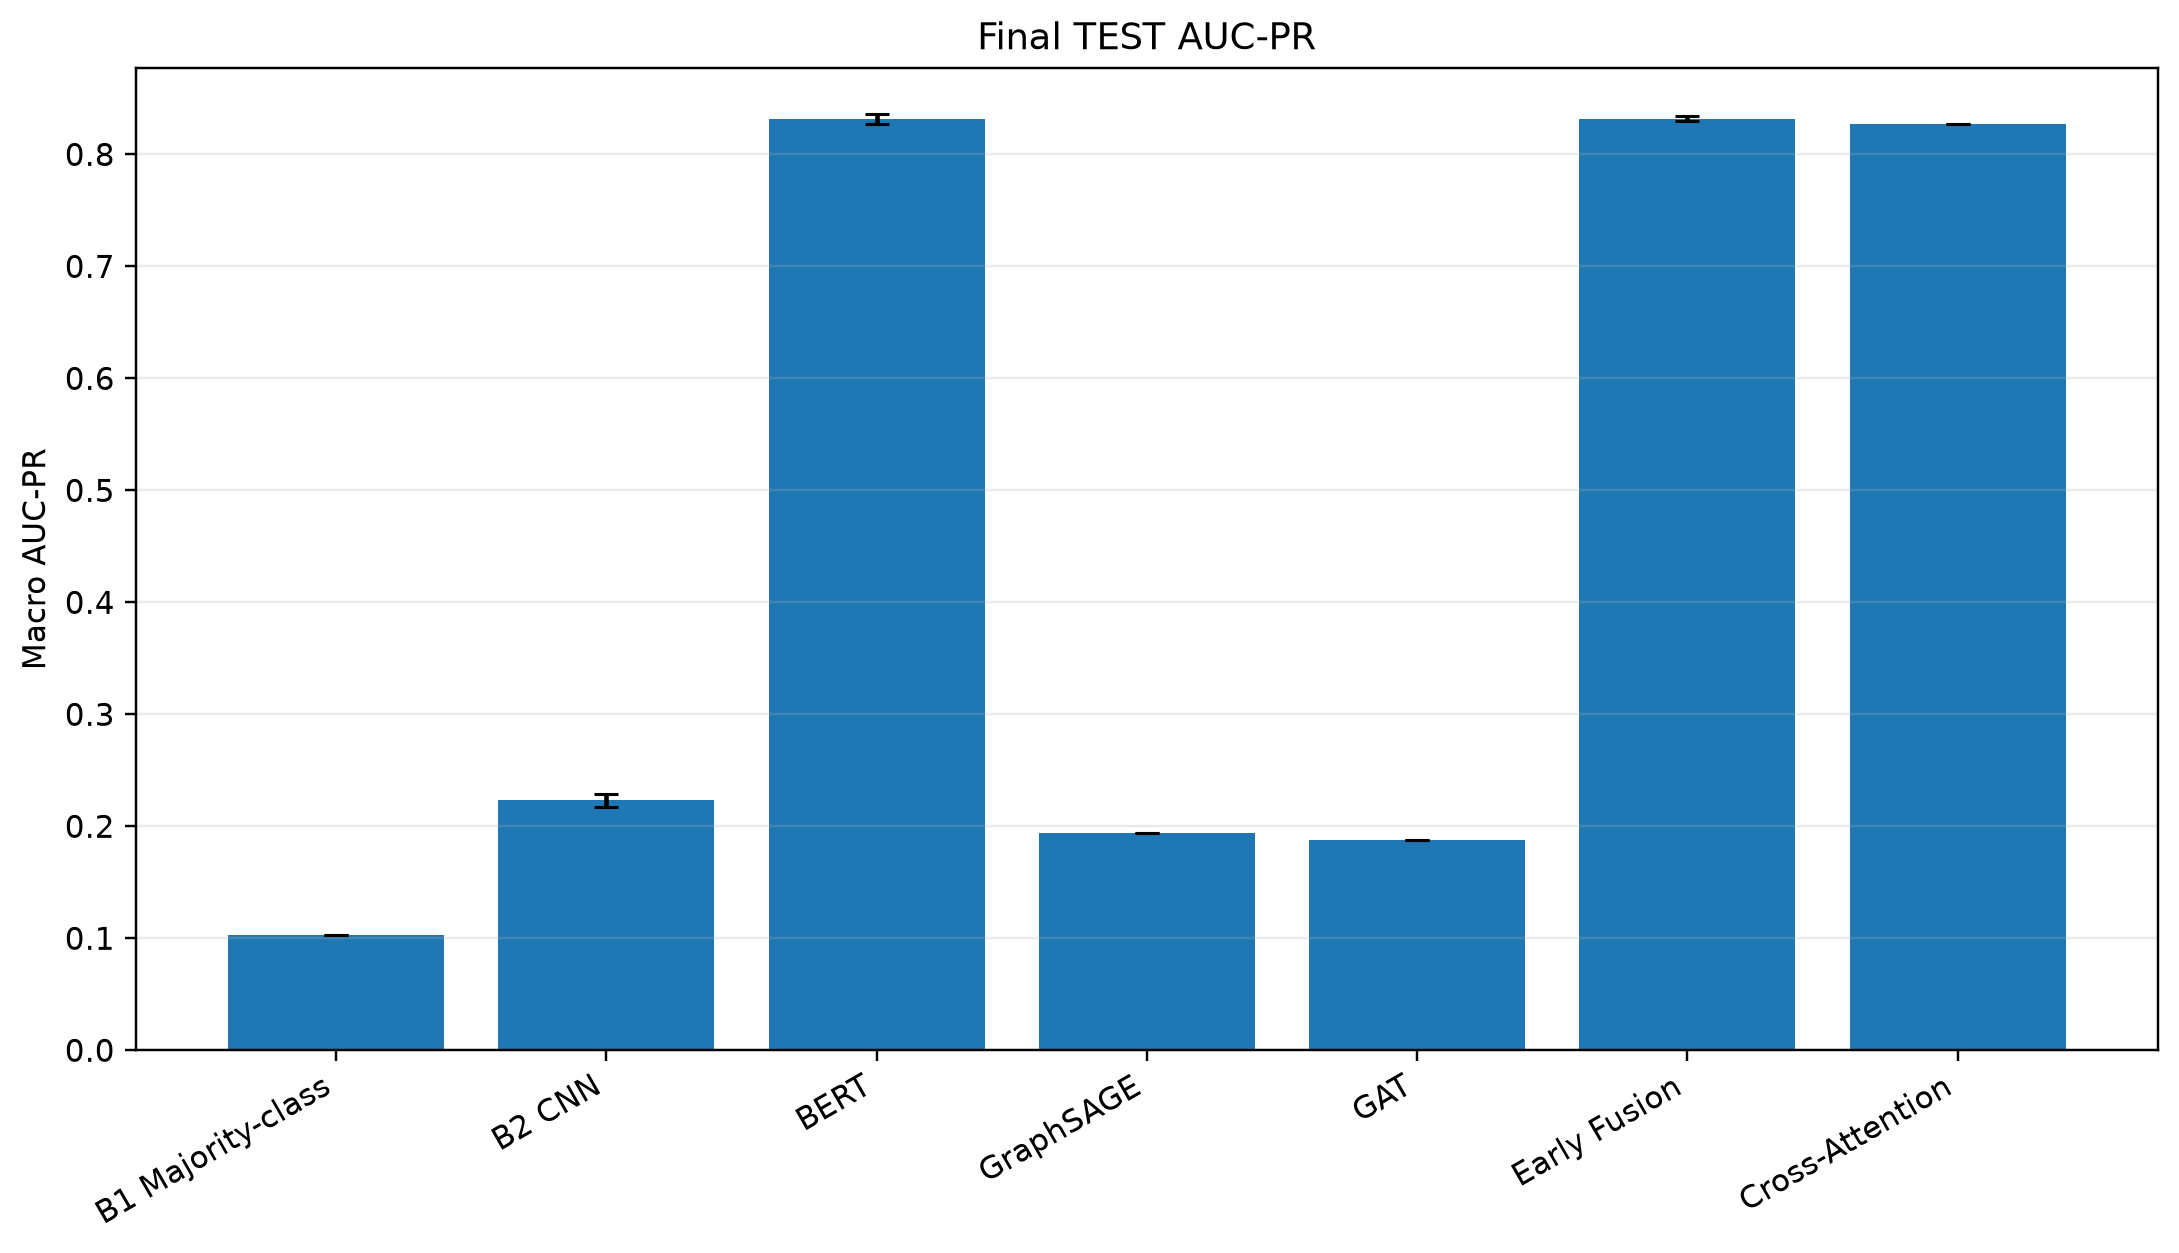
\includegraphics[width=\linewidth]{figure_final_auc_pr.png}
\caption{Supplied final TEST comparison. ``AUC-PR'' denotes Macro AP. Seed SD is estimable only for the three-run models in Table~\ref{tab:test}; visually negligible bars for single-run models do not demonstrate zero variability.}\label{fig:test}
\end{figure}

Label-specific exploratory effects vary. The largest reported gain is passionate (+0.046097 AP), while acoustic drums decreases by 0.063072. Such post-hoc differences describe this saved evaluation, not confirmed label-level improvements. The three supplied classification cases in Table~\ref{tab:cases} include a shared success, a shared miss, and an additional fusion error. They illustrate behavior without selecting a more favorable model or threshold.

\subsection{Task 4: Retrieval and prototype readout}
At seed 42, T4-B validation $mR=0.09273670$ exceeds T4-A's 0.07328145. Across three seeds, selected T4-B validation mR is $0.09554691\pm0.00225169$ (population SD). Final TEST mR is $0.0796\pm0.0065$, with all six directional recalls shown in Table~\ref{tab:retrieval} and Figure~\ref{fig:retrieval}. The mean is approximately $7.7\times$ random mR over the identical 514-item pool, demonstrating learned alignment. The validation-to-TEST decline and approximately 2\% exact-pair R@1 limit any claim of retrieval quality.
\begin{table}[t]\centering\small
\caption{Task-4 three-seed TEST retrieval. Recalls are means; mR uncertainty is population SD.}\label{tab:retrieval}
\begin{tabular}{@{}lrrr@{}}\toprule
Direction & R@1 & R@5 & R@10\\\midrule
Audio $\to$ caption & $\sim$0.0227 & 0.0856 & 0.1368\\
Caption $\to$ audio & $\sim$0.0195 & 0.0707 & 0.1420\\\midrule
\multicolumn{2}{@{}l}{Learned mR} & \multicolumn{2}{r@{}}{$0.0796\pm0.0065$}\\
\multicolumn{2}{@{}l}{Random mR, 514 candidates} & \multicolumn{2}{r@{}}{$\sim$0.0104}\\\bottomrule
\end{tabular}
\end{table}
\begin{figure}[t]\centering
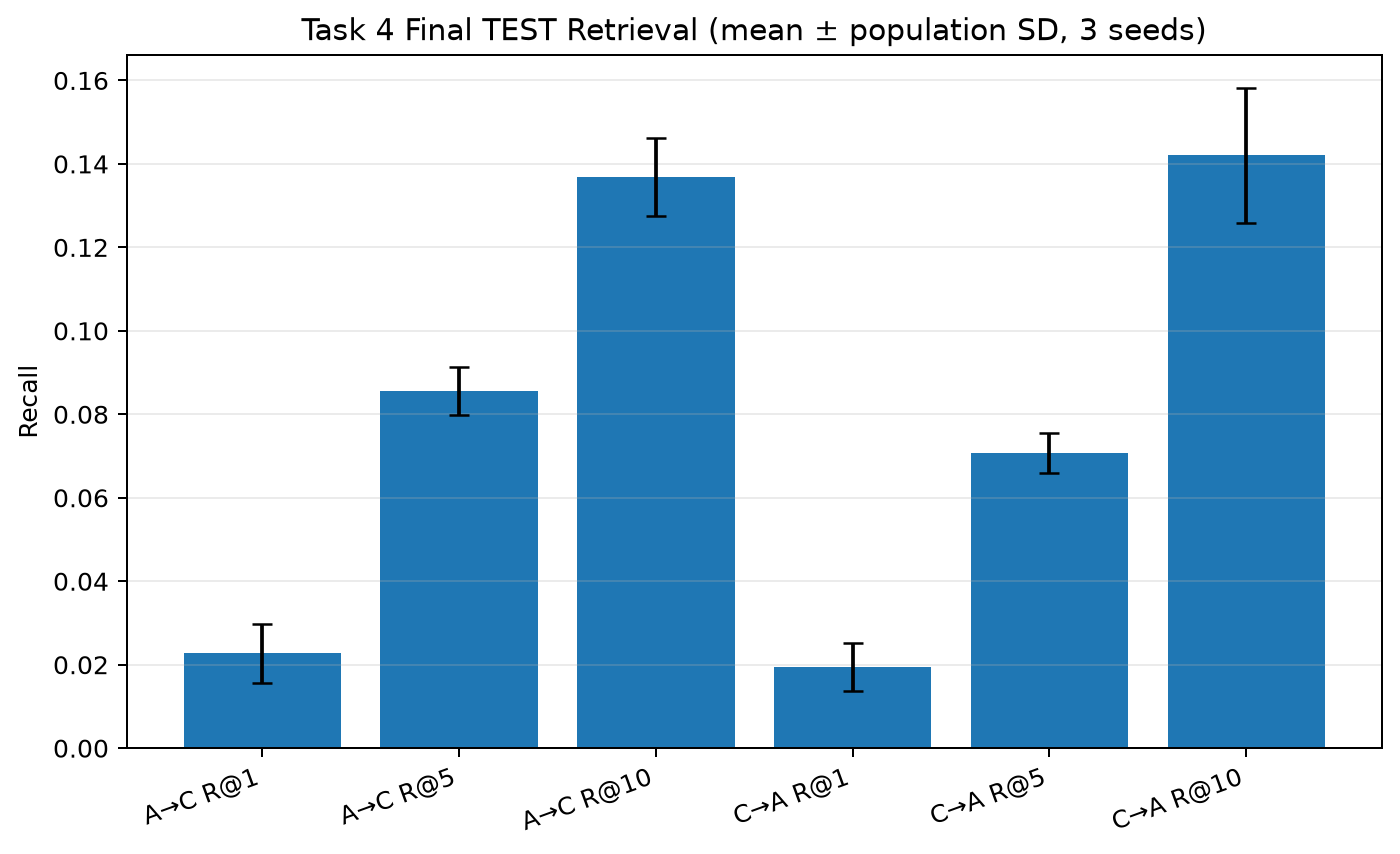
\includegraphics[width=\linewidth]{task4_test_recall_at_k.png}
\caption{Supplied bidirectional TEST retrieval plot for T4-B. Exact matching remains modest despite improvement over random ranking.}\label{fig:retrieval}
\end{figure}

Table~\ref{tab:prototype} reports the tag-prototype results. Caption-to-label AP is higher than audio-to-label AP, but both are well below supervised Task 3. These results measure prototype compatibility after supervised initialization; they do not show that unseen labels emerged from tag-free pretraining.
\begin{table}[t]\centering\small
\caption{TEST tag readout, mean $\pm$ population SD for Task 4. The supervised reference is shown for comparison.}\label{tab:prototype}
\begin{tabular}{@{}lr@{}}\toprule
Readout & Macro AP\\\midrule
Caption $\to$ label text & $0.274\pm0.022$\\
Audio $\to$ label text & $0.146\pm0.006$\\
Task-3 supervised reference & 0.832\\\bottomrule
\end{tabular}
\end{table}

\subsection{Human evaluation}
The pooled score is 3.02/5 with sample SD approximately 1.58, consistent with moderate but variable semantic match. Figure~\ref{fig:human} and Table~\ref{tab:human} expose the variation rather than reporting only the mean. Q06 receives five ratings of 5, while Q01 and Q08 average 1.2. Q04 and Q10 span the full scale. The mean of listener means is also 3.02, with sample SD 0.6140 across five listeners; this is different from the pooled SD. Fifty ratings are repeated assessments of ten queries by five listeners, not 50 independent listeners or queries.
\begin{figure}[t]\centering
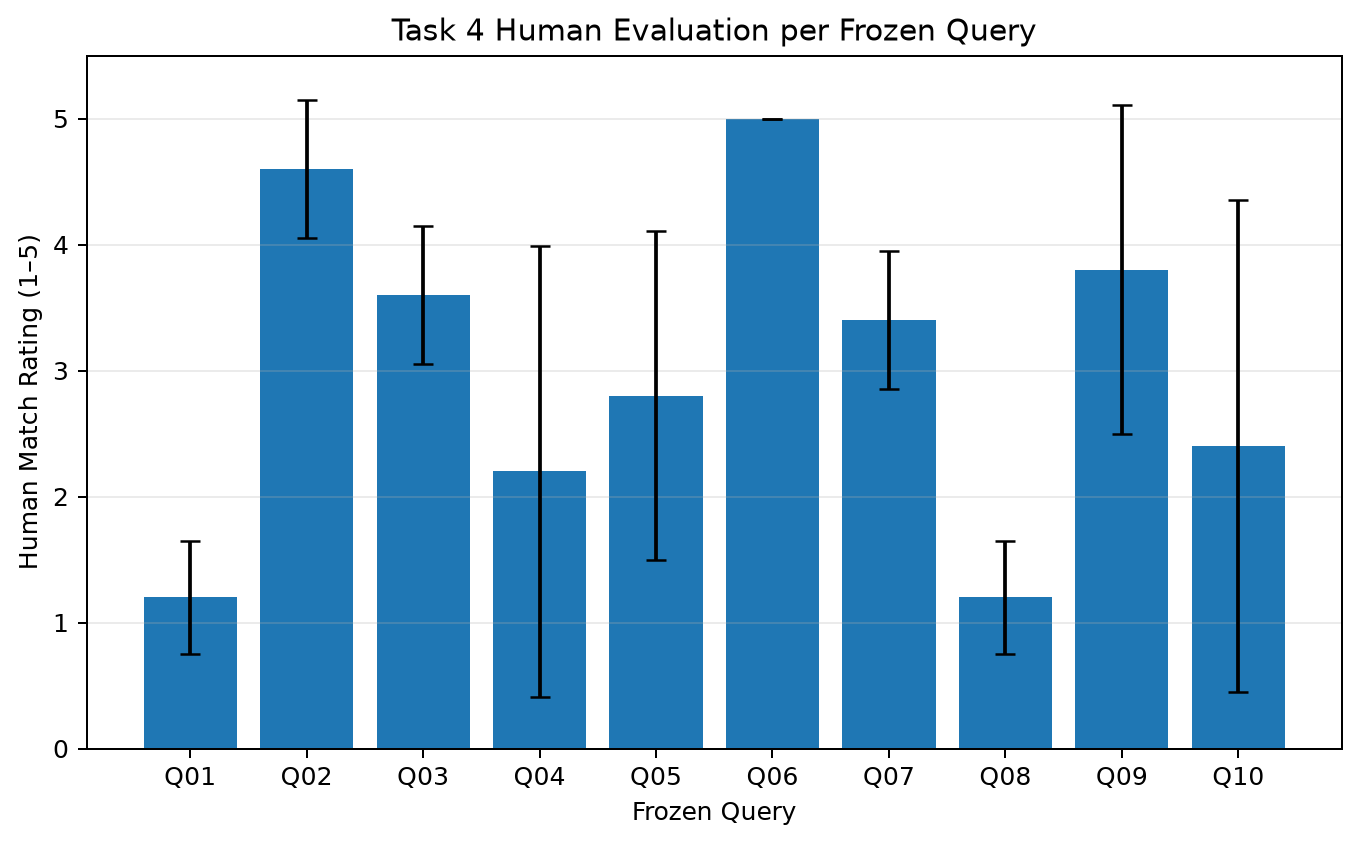
\includegraphics[width=\linewidth]{task4_human_ratings.png}
\caption{Supplied listener ratings for the ten fixed caption-to-audio top-one retrievals. The study is descriptive and small; variability does not support a population-level quality claim.}\label{fig:human}
\end{figure}

\section{Discussion}\label{sec:discussion}
The implemented text pipeline is much more predictive than the audio-only pipelines on these MusicCaps-derived labels. However, BERT receives both substantial external pretraining and rich human-written descriptions, while graph models summarize only ten seconds of audio into nine mean-pooled nodes. The comparison holds tracks, splits, and targets fixed, but does not isolate modality from information content and pretraining. The observed ordering should therefore remain specific to this experimental design.

The fusion result answers the central question directly: additional graph audio does not establish a reliable overall gain over BERT. Small positive and negative label-level changes can coexist with near-identical aggregate performance. This finding is useful because it identifies where future work must add information beyond what captions already reveal. More complex fusion alone is not demonstrated to solve the problem; M4 also trails M3 in validation.

Retrieval asks a distinct question and provides complementary evidence. Above-chance exact-pair retrieval demonstrates that the shared space contains pair-relevant information. At the same time, two music clips can match the same description without being the designated pair, so semantic ratings and exact-pair recalls need not coincide. The listening results are compatible with this distinction, but the limited study cannot quantify its contribution to retrieval errors. The prototype results further show that paired alignment does not automatically recover the decision boundaries of the supervised classifier.

\section{Limitations and Threats to Validity}\label{sec:limits}
\textbf{Caption--target circularity.} The 20 labels originate in MusicCaps aspect lists, while BERT consumes semantically related captions. Caption/aspect independence and lexical or synonym coverage are \emph{not verified from available project evidence}. Strong BERT AP may partly measure text-to-tag extraction. No lexical baseline or read-only overlap audit is available to resolve that interpretation.

\textbf{Dataset coverage and isolation.} The 381 excluded clips may create availability-selection bias; its distributional impact is unquantified. Track/source identity checks do not establish artist or recording-level near-duplicate isolation across splits. Using only MusicCaps limits generalization and differs from the brief's Task-2/3 dataset suggestions. No emotion regression is evaluated.

\textbf{Representation and comparison scope.} Nine mean-pooled nodes can discard local acoustic detail retained by a spectrogram CNN. GAT/G1 is absent, so graph-topology claims are limited to tested comparisons. Pooled cross-attention cannot establish segment-to-word alignment, and neither topology plots nor attention scores alone establish causal musical explanations. BERT's pretraining and caption access prevent a modality-only interpretation. CNN's best epoch lies at its budget ceiling, and the F1 threshold grid has an upper-bound optimum for BERT/M3.

\textbf{Seed and numerical uncertainty.} Three seeds provide limited precision and may share selected upstream initialization. The exploratory bootstrap is post-hoc and does not establish fusion superiority. Frozen weights can still produce stochastic activations through dropout. Rank-boundary floating-point sensitivity was observed during Task-4 validation rechecks; differences below one-query recall resolution should not be overinterpreted. Strict-greater ranking is mildly optimistic for exact ties.

\textbf{Contrastive and human interpretation.} InfoNCE treats other batch items as negatives even when musically similar. Exact-pair metrics penalize plausible alternatives. Prototype readout inherits tag-supervised encoders and is not strict label-naive zero-shot learning. Five listeners and ten fixed queries support descriptive conclusions only; a robust inter-rater reliability analysis is absent. The provided HTML records a listening instruction, not proof of playback compliance.

\textbf{Provenance coverage.} The independent audit cannot certify the full source of nine scripts (07--12, 18, 62, 63). Git commit, full environment, and some training hyperparameters are unavailable. The Task-3 comparator in Task-4 consolidation is report-level rather than fully linked through the Task-4 hash chain; the separate Task-3 final JSON independently supplies the same value. Supplied case-study assets are available at result level, but this does not retroactively certify Scripts 62--63.

\section{Conclusion and Future Work}\label{sec:conclusion}
The project establishes a controlled four-task comparison on a frozen 5,140-clip MusicCaps corpus. Fine-tuned BERT is a strong predictor of the aspect-derived targets. Early Fusion recovers approximately the same overall performance and does not reliably surpass it. Contrastive graph--text training learns alignment substantially above random retrieval, while exact-pair accuracy remains modest and human match quality varies. Prototype-based tag readout underperforms supervised classification and requires explicit qualification because of supervised initialization.

The highest-priority next analysis is a read-only caption--label overlap audit with a lexical baseline, followed by recording-duplicate analysis on the existing split. Separate future experiments could test richer temporal audio features, compare GAT on both graph types, and evaluate a label-naive contrastive initialization. A larger listening study with reliability analysis would better characterize semantic retrieval. These additions should be preregistered as new analyses or experiments, preserving the completed results and avoiding post-TEST reselection.

\bibliographystyle{IEEEtran}
\bibliography{references}

\clearpage
\onecolumn
\appendices
\section{Audit, Configuration, and Qualitative Evidence}\label{sec:appendix}
Table~\ref{tab:audit} summarizes the 76-script audit. ``Not verified'' marks a source-evidence limit, not a confirmed failure. The nine minor-fix entries are 27, 57--59, 61, 68, 70, 73, and 76; Script 25 is redundant. The audit contains the full per-script dispositions.
\begin{table}[!ht]\centering\small
\caption{Final audit disposition of 76 scripts.}\label{tab:audit}
\begin{tabular}{@{}lr@{}}\toprule
Disposition & Count\\\midrule
KEEP & 57\\
MINOR FIX & 9\\
REDUNDANT & 1\\
NOT VERIFIED FROM AVAILABLE EVIDENCE & 9\\
MAJOR FIX / REPLACE & 0 confirmed\\\midrule
Total & 76\\\bottomrule
\end{tabular}
\end{table}

The frozen label order is: low quality; instrumental; medium tempo; fast tempo; noisy; emotional; energetic; passionate; amateur recording; bass guitar; electric guitar; live performance; slow tempo; male vocal; mono; acoustic drums; groovy; no voices; acoustic guitar; piano. Table~\ref{tab:config} gathers additional supported settings. Missing optimizer details are not replaced with assumed defaults.
\begin{table}[!ht]\centering\small
\caption{Additional audited configuration.}\label{tab:config}
\begin{tabular}{@{}ll@{}}\toprule
Component & Setting\\\midrule
BERT classifier & CLS, $768\to20$\\
GAT input / pooled output & 64 / 128 dimensions\\
GAT heads / attention dropout & 4 / 0.2\\
G2 cosine cutoff / extra degree & $>0.85$ / 2\\
M3 projections / hidden / dropout & 256 / 256 / 0.2\\
Task-4 embedding / batch & 256 / 32\\
Task-4 temperature & 0.07\\
T4-B trainable BERT layers & 10--11\\
T4-B trainable GAT layer & GAT3\\
Final seed set & 42, 1337, 2026\\\bottomrule
\end{tabular}
\end{table}

\begin{table*}[!ht]\centering\small
\caption{Three supplied post-hoc classification examples, using frozen predictions. The graph in Figure~\ref{fig:graph} belongs to the third case. These are label-level cases; complete caption/graph-path alignment evidence was not supplied.}\label{tab:cases}
\begin{tabular}{@{}p{.24\textwidth}p{.18\textwidth}p{.22\textwidth}p{.25\textwidth}@{}}\toprule
Track / case & True labels & BERT predictions & M3 predictions\\\midrule
\texttt{mc\_PIIAyM4H1UE\_100\_110}\newline High-confidence correct & instrumental & instrumental & instrumental\\
\texttt{mc\_yuWjB3XA8tc\_480\_490}\newline High-confidence incorrect & live performance & none & none\\
\texttt{mc\_RFbWkL818XQ\_30\_40}\newline Near threshold & instrumental; medium tempo & instrumental; medium tempo; energetic & instrumental; medium tempo; energetic; groovy\\\bottomrule
\end{tabular}
\end{table*}

\begin{table}[!ht]\centering\small
\caption{Human ratings by fixed query: five listeners per item. SD is sample SD; descriptors summarize the questionnaire caption, not the retrieved audio.}\label{tab:human}
\begin{tabular}{@{}llrrr@{}}\toprule
ID & Caption topic & Mean & SD & Range\\\midrule
Q01 & Om mantra & 1.2 & 0.4472 & 1--2\\
Q02 & Electronic shuffle & 4.6 & 0.5477 & 4--5\\
Q03 & Group singing/guitar & 3.6 & 0.5477 & 3--4\\
Q04 & Song/vehicle sounds & 2.2 & 1.7889 & 1--5\\
Q05 & Duet/harp & 2.8 & 1.3038 & 1--4\\
Q06 & Electronic dance & 5.0 & 0.0000 & 5--5\\
Q07 & Unison voices/sitar & 3.4 & 0.5477 & 3--4\\
Q08 & Devotional music & 1.2 & 0.4472 & 1--2\\
Q09 & Scratching/hip-hop & 3.8 & 1.3038 & 2--5\\
Q10 & Brass/clicking & 2.4 & 1.9494 & 1--5\\\bottomrule
\end{tabular}
\end{table}

\section{Artifact Provenance}\label{sec:provenance}
The report uses the independent audit for implementation and workflow claims, the assignment for intended requirements, and the supplied JSON/CSV files for frozen quantitative results. The original result files remain unchanged. In particular, saved ``auc\_pr'' fields are interpreted using the explicit mean-AP definition in \texttt{final\_test\_evaluation.json}. Task-4 human-study documentation combines its frozen summary with the supplied \texttt{index.html} questionnaire.

The pretraining lock SHA256 is \texttt{caffa90d9de726a6\allowbreak a28fb15b2ee0e28f\allowbreak 4abac8f0766c90d5\allowbreak b0e027a6c917b4e8}. The Task-3 evaluation hash recorded by the asset manifest is \texttt{8c6db5aed0cd23b7\allowbreak 300da3b403089e70\allowbreak 48f7f4ffcb64dcb8\allowbreak f3d1f555bd59f35d}. The Task-4 audit hash recorded by its summary is \texttt{712bb131762a9791\allowbreak 550db2a4b98aa271\allowbreak 824c9c878f54d9ef\allowbreak 7fe4917c846a3413}. These are provenance identities from the supplied artifacts, not a claim that all upstream checkpoints were available for independent inspection. The reporting package includes a separate asset-access/hash check, distinguishing locally verified files from upstream records.
\end{document}
